\documentclass[aps,prb,groupedaddress,nofootinbib,floatfix]{revtex4}
\usepackage{graphicx}
\usepackage{graphics}
\usepackage{epsfig}
\usepackage{url}
\usepackage[utf8]{inputenc}
\usepackage[T1]{fontenc}
\usepackage{textcomp}
\usepackage{amsmath, amssymb}
\usepackage[at]{easylist}
\usepackage{soul}
\usepackage{listings}
\usepackage{color}

\definecolor{blue-violet}{rgb}{0.54, 0.17, 0.89}
\definecolor{bondiblue}{rgb}{0.0,0.58,0.71}
\definecolor{bronze}{rgb}{0.8,0.5,0.2}
\definecolor{applegreen}{rgb}{0.55,0.71,0.0}
\definecolor{arylideyellow}{rgb}{0.91,0.84,0.42}
\definecolor{grey}{rgb}{0.52,0.52,0.51}

\lstset{
	language=Python,
	aboveskip=3mm,
	belowskip=3mm,
	basicstyle={\small\ttfamily},
	numberstyle=\color{arylideyellow},
	keywordstyle=\color{bondiblue},
	commentstyle=\color{bronze},
	stringstyle=\color{applegreen},
	breaklines=true,
	showstringspaces=false,
	breakatwhitespace=true,
	tabsize=3
}
	



\pdfsuppresswarningpagegroup=1

\begin{document}
\author{Preston Seligman}
\title{Numerical Integration}
\date{February 20, 2025}
\maketitle
\section*{Overview}
In this homework, different numerical integration methods were used to determine their error. The Trapezoid Rule, Simpson's Method, and Romberg Extrapolation were examined on two different functions to determine the error in integration values over N points. Results were obtained for each method using both $10^5 \text{and} 10^7$ values for N. 
\paragraph{Theoretical Framework} 
For computational analysis, it is not possible to integrate over infinitely many points. As the $\lim_{h \to 0} ,\text{machine precision} \varepsilon_{m}$ limits the computational ability. Therefore, a method of approximation is needed. For integrating a function $f(x)$ on a continuous interval between $[a,b]$, approximations for the area under a curve can be made. 
The most basic form of approximation is the \ul{Trapezoid Rule}, given by \[
	\int_{a}^{b} f(x)dx \simeq \frac{h}{2}f_{1}+hf_{2}+hf_{3}\ldots+hf_{N-1}+\frac{h}{2}f_{N}, \varepsilon_{t} = O(\frac{[b-a]^3}{N^{2}})f^{2} 
.\] 
in the interval $[a,b]$ for N points spaced an equal distance h apart. Here,  $\varepsilon_{t}$ is the error in the Trapezoid method (using big O notation.)
Expanding upon the Trapezoid Rule, \ul{Simpson's Rule} can be obtained by fitting the integrand $f(x)$ to a parabola over each equally spaced interval. This yields  \[
	\int_{a}^{b} f(x)dx \simeq \frac{h}{3}f_{1}+\frac{4h}{3}f_{2}+\frac{2h}{3}f_{3}+\frac{4h}{3}f_{4}\ldots+\frac{4h}{3}f_{N-1}+\frac{h}{3}f_{N}, \varepsilon_{s}=O(\frac{[b-a]^5}{N^{4}})f^{4} 
.\] 
for N points spaced equal distance h apart, and $\varepsilon_{s}$ is error in the Simpson Rule.
Further extrapolation can be done by setting the normal value used for h to be $\frac{h}{2}$. Such an extrapolation yields the Romberg Extrapolation, where doing so yields \[
	R_{t} \simeq \frac{4}{3}A(\frac{h}{2}) - \frac{1}{3}A(h), R_{s} \simeq \frac{16}{15}A(\frac{h}{2})-\frac{1}{15}A(h)
.\] 
where A is the area computed for the given height value. An in-depth derivation of the Romberg Extrapolation for Simpson's Rule will be shown later.
\paragraph{Code} 
The code used for this analysis is as follows:
\begin{lstlisting}
import matplotlib.pyplot as plt 
import numpy as np
import scipy.optimize as opt

def func(x):          # function to be integrated
    return np.exp(-x)

def trapezoid(A,B,N):   #integrate from A to B using N points
    h = (B - A)/(N - 1)                     # step size 
    sum = (func(A)+func(B))/2               # (1st + last)/2
    for i in range(1, N-1):        # i goes from 1 to (N-1)-1
       sum += func(A+i*h)
#       sum=np.float32(sum)            # to simulate single-precision (32 bit) calculation
    return h*sum  

def simpson(A,B,N):
    if ((N-1)%2==1):     #  if number of intervals odd
        print("Simpson's rule requires even number of intervals")
        return 0
    h = (B - A)/(N - 1)                     # step size 
    sum = (func(A)+func(B))/3               # (1st + last)/3
    for i in range(1, N-1,2):        # i loops over odd integers  from 1 to (N-1)-1
       sum += 4/3*func(A+i*h)
 #      sum=np.float32(sum)
    for i in range(2, N-1,2):        # i loops over even integers starting with 2
       sum += 2/3*func(A+i*h)
#       sum=np.float32(sum)
    return h*sum  
def romberg(A,B,N):
    return (((16.0 *simpson(A, B, 2*N-1))-simpson(A, B, N))/15.0)
A = 0.0
B = 1.0

maxpoints = 10**5
#%%
Nvalues = []    #empty lists
traperror = []
simperr = []
romberr = []
#%%
exact = 1-np.exp(-1)

N=3
while N<maxpoints:    # loop over number of points
    print(N)    #just so you can see while code is running
    Nvalues.append(N)
    traperror.append(abs(trapezoid(A,B,N)-exact)/exact) # Error in trapezoid method
    simperr.append(abs(simpson(A,B,N)-exact)/exact)
    romberr.append(abs(romberg(A, B, N)-exact)/exact)
    N=int(N*1.1)+1    # N grows roughly by 1.1 factor each time
    if N%2 == 0:
        N=N+1    # make sure N is odd
# %%
def fit(x,s):
    return s*x
trapfit_data = traperror[0:16]
simpfit_data = simperr[0:16]
rombfit_data = romberr[0:16]
trapfit, trapcovar=opt.curve_fit(fit, Nvalues, traperror)
simpfit, simpcovar=opt.curve_fit(fit, Nvalues, simperr)
rombfit, rombcovar =opt.curve_fit(fit, Nvalues, romberr)
Narray = np.array(Nvalues)
print(trapfit,simpfit,rombfit)

#%%
plt.loglog(Nvalues,traperror,label="Trapezoid Error", linewidth=2.5)   # log log plot of error in trapezoid method
plt.loglog(Nvalues, simperr, label="Simpson Error", linewidth=2.5) 
plt.loglog(Nvalues,romberr, label="Romberg Error", linewidth=2.5, linestyle="solid")
plt.loglog(Nvalues, 0.1/(Narray**2), label=r"$\frac{0.1}{N^{2}}$", linestyle = "dashed", linewidth=1.5)
plt.loglog(Nvalues, 0.01/(Narray**4), label=r"$\frac{0.01}{N^{4}}$", linestyle = "dashed", linewidth=1.5)
plt.loglog(Nvalues, 0.0001/(Narray**6), label=r"$\frac{0.0001}{N^{6}}$", linestyle = "dashed", linewidth=1.5)
plt.loglog(Nvalues, 10e-17*(Narray**0.5), label=r"$10^{-17}N^{\frac{1}{2}}$", linestyle="dashed", linewidth=1.5)
plt.ylim([1e-17,1e-1])   # set range of y values
legend = plt.legend(loc="upper right", fontsize = 8)
plt.title(r"Integration on $f(x)=e^{-x}$", fontsize = 18)
plt.xlabel("Number of Points (N)", fontsize = 14)
plt.ylabel("Error", fontsize = 14)
plt.show()    #show the graph
# %%
\end{lstlisting}
This code contains all the parts used for this assignment. 
\section*{Problems}
\subsection*{Problem 1}
An initial run of the Trapezoid and Simpson's Rule was performed for the function $f(x)=e^{-x}$ on the interval $[0,1]$. Results were gathered using $N=10^{5} \text{and} 10^{7}$ points for integration. Results are shown in \ref{fig:Plot1} and \ref{fig:Plot2}. 
\begin{figure}
	\begin{minipage}[c]{0.4\linewidth}
		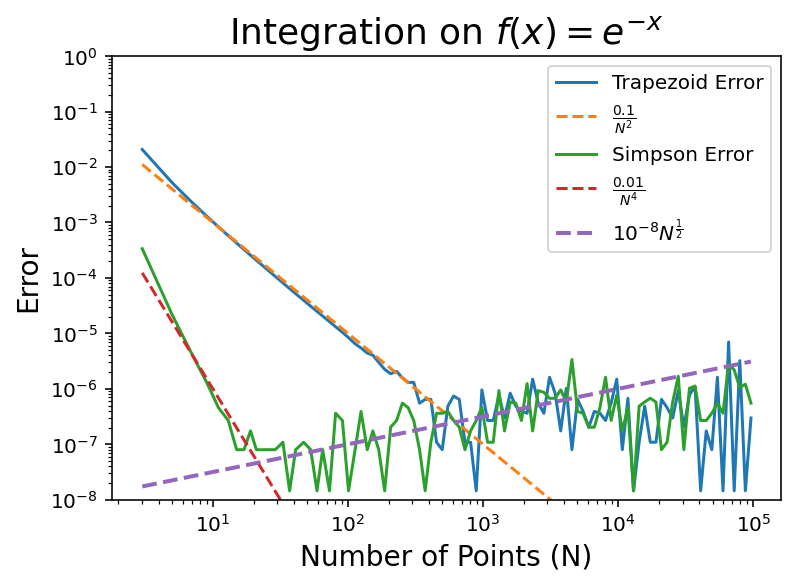
\includegraphics[width=\linewidth]{Plot1(10^5).png}
		\caption{Single-precision plot on range $N=10^{5}$ }
		\label{fig:Plot1}
	\end{minipage}
	\begin{minipage}[c]{0.4\linewidth}
		\includegraphics[width=\linewidth]{Plot1(10^7).png}
		\caption{Single-precision plot on range $N=10^{7}$ }
		\label{fig:Plot2}
	\end{minipage}
\end{figure}
As can be seen, the error for Simpson's rule reduces for faster (that is, for fewer iterations of N) until reaching the limit for machine precision. Here, since single-precision was used, this is $\varepsilon_{m} \simeq 10^{-8}$. As can be seen from the data, once both Simpson error and Trapezoid error reach this limit, their error fluctuates around the line graphed by $10^{-8}N^{\frac{1}{2}}$. 
The power law dependence for both Simpson's Rule and the Trapezoid rule were also determined. From literature, these values are $\frac{1}{N^{2}}$ for the Trapezoid rule and $\frac{1}{N^{4}}$ for Simpson's Rule, respectively. Initial application of this power-law dependence did not align with the obtained values, however. In this data collection, the Trapezoid rule more closely resembled $\frac{0.1}{N^{2}}$ and $\frac{0.01}{N^{4}}$ for Simpson's rule. This is likely due to the fact that the real calculation for relative error includes a term for h. Therefore, the algorithmic error is only approximated by the reported values and needs to be further determined.
\subsection*{Problem 2}
Modifying the code to use double precision, we find that $\varepsilon_{m} \simeq 10^{-17}$. Results can be seen as before for Problem 1.
\begin{figure}
	\begin{minipage}[c]{0.4\linewidth}
		\includegraphics[width=\linewidth]{Plot2(10^5).png}
		\caption{Double-precision plot on range $N=10^{5}$ }
		\label{fig:Plot3}
	\end{minipage}
	\begin{minipage}[c]{0.4\linewidth}
		\includegraphics[width=\linewidth]{Plot2(10^7).png}
		\caption{Double-precision plot on range $N=10^{7}$ }
		\label{fig:Plot4}
	\end{minipage}
\end{figure}
Comparing values from Figures \ref{fig:Plot3} and \ref{fig:Plot4} to their equivalents form Figures \ref{fig:Plot1} and \ref{fig:Plot2}, we find that double precision yields far more precise results, with much lower error values. Total error is reduced for both methods, as machine error is now lower. However, no change in algorithmic error is made, as evidenced by the same power-law dependence as Problem 1. Moreover, we see that it takes both methods greater iterations over N to approach the machine error limit. 
\subsection*{Problem 3} 
Now, both Simpson and Trapezoid rule are being used to integrate the function $sin(e^{5}x+7)$ over the interval $[0,1]$. As before, plots are shown.
\begin{figure}
	\begin{minipage}[c]{0.4\linewidth}
		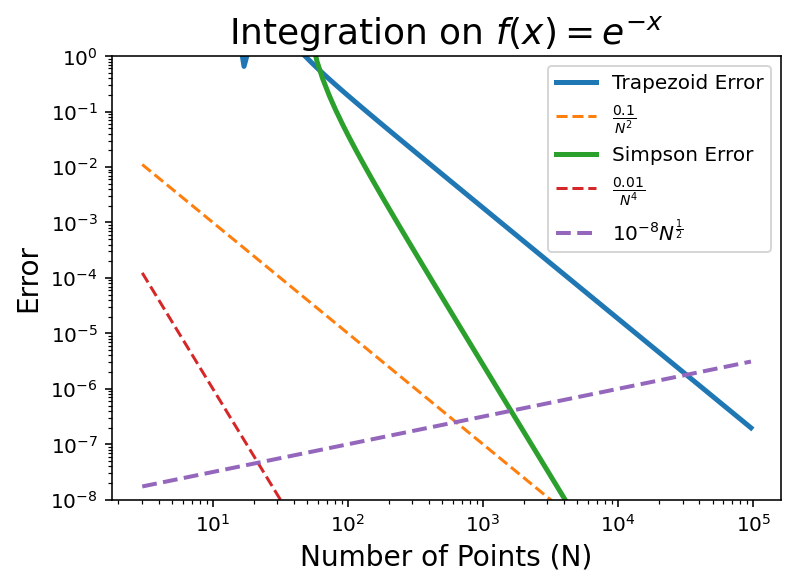
\includegraphics[width=\linewidth]{Plot3(10^5).png}
		\caption{Plot on range $N=10^{5}$ }
		\label{fig:Plot5}
	\end{minipage}
	\begin{minipage}[c]{0.4\linewidth}
		\includegraphics[width=\linewidth]{Plot3(10^7).png}
		\caption{Plot on range $N=10^{7}$ }
		\label{fig:Plot6}
	\end{minipage}
\end{figure}
As evidenced from above, error behavior differs here when compared with the function $f(x)=e^{-x}$. Error in the trapezoid rule scales as $\frac{f''}{f}$ which is much greater for this function than for the previous function. Therefore, the error will not scale exactly as $\frac{1}{N^{2}}$, however its slope should be the same. Importantly, the error does not begin decreasing until 25 iterations, with the error in both methods remaining high. This is in contrast with the scaling for the function $f(x)=e^{-x}$, where the error for both methods begins decreasing far sooner. For both methods, the error scaling for this function is higher than previous.
\subsection*{Problem 4} 
Applying Romberg extrapolation to Simpson's Rule, we find
\begin{align*}
	I_{Simp}(h) & = I + \alpha h^{4} + \beta h^{6}\\
	I_{Romb}(\frac{h}{2}) & = I + \alpha (\frac{h}{2})^{4} + \beta (\frac{h}{2})^{6}\\
\end{align*}
Combining these equations to solve for to eliminate $\alpha$
\begin{align*}
	16I_{Romb}(\frac{h}{2})&-I_{Trap}(h)\\
	I &= \frac{16}{15}I(\frac{h}{2})-\frac{1}{15}I(h)+\beta(h^{6})
\end{align*}
Using this, a Romberg extrapolation can be performed on the function $f(x)=e^{-x}$, which yields the following plots:
\begin{figure}
	\begin{minipage}[c]{0.4\linewidth}
		\includegraphics[width=\linewidth]{Plot4(10^5).png}
		\caption{Romberg extrapolation on range $N=10^{5}$ }
		\label{fig:Plot7}
	\end{minipage}
	\begin{minipage}[c]{0.4\linewidth}
		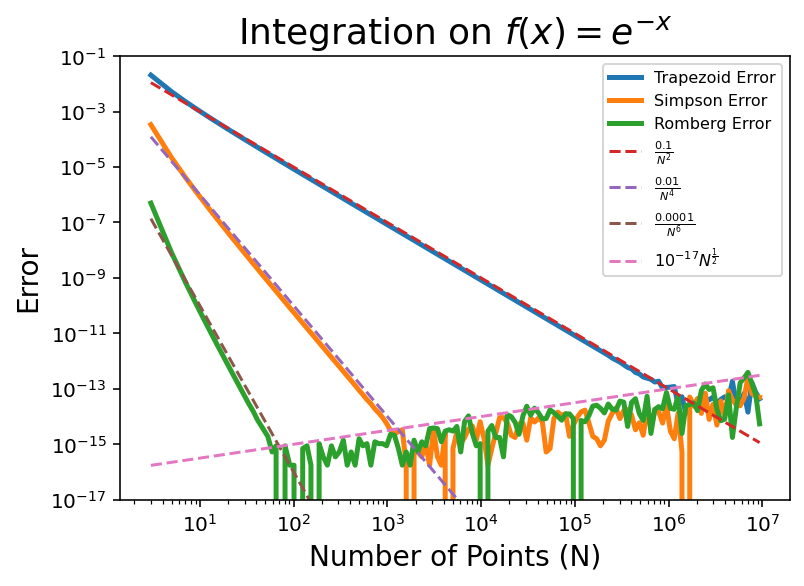
\includegraphics[width=\linewidth]{Plot4(10^7).png}
		\caption{Romberg extrapolation on range $N=10^{7}$ }
		\label{fig:Plot8}
	\end{minipage}
\end{figure}
Romberg error scales by a function $\frac{f}{N^{6}}$. The exact scaling function could not be determined, however it appears close to $\frac{0.0001}{N^{6}}$. Romberg error therefore decreases far faster than both Simpson's and Trapezoid rule over the same interval. Romberg extrapolation has a faster decreasing error, and therefore requires fewer iterations over N before reaching limit due to machine precision.
\end{document}
